% Figure 1: per-record (PR) versus device-signed Merkle root (DR). Compile: pdflatex fig1_designs.tex
\documentclass[tikz,border=2pt]{standalone}
\usepackage{mathptmx}
\usetikzlibrary{positioning,arrows.meta,calc,fit,backgrounds}
\definecolor{okblue}{HTML}{0072B2}
\definecolor{okorange}{HTML}{E69F00}
\definecolor{okgreen}{HTML}{009E73}
\definecolor{okverm}{HTML}{D55E00}
\begin{document}
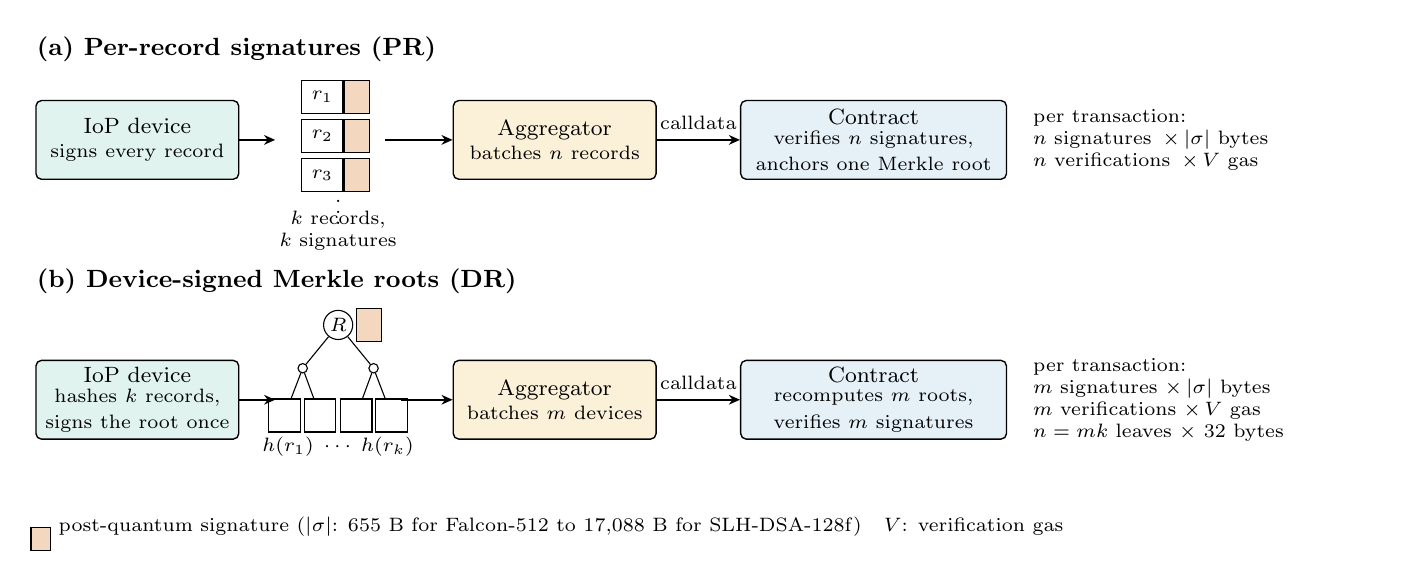
\begin{tikzpicture}[
  font=\footnotesize, >={Stealth[length=4pt,width=3.5pt]},
  box/.style={draw, rounded corners=2pt, align=center, minimum height=10mm, inner sep=2.5pt, line width=0.5pt, text width=#1},
  box/.default=30mm,
  rec/.style={draw, fill=white, minimum width=5.2mm, minimum height=4.2mm, inner sep=0pt, font=\scriptsize, line width=0.4pt},
  sig/.style={draw, fill=okverm!25, minimum width=3.2mm, minimum height=4.2mm, inner sep=0pt, line width=0.4pt},
  flow/.style={->, line width=0.7pt},
  lab/.style={font=\scriptsize, align=center},
  cost/.style={font=\scriptsize, align=left, text width=44mm, inner sep=2pt},
]
% ============================================================ (a) per-record
\node[font=\small\bfseries, anchor=west] at (-0.2,1.15) {(a) Per-record signatures (PR)};
\node[box=24mm, fill=okgreen!12] (devA) at (1.2,0) {IoP device\\[-1pt]{\scriptsize signs every record}};
% records with signatures
\foreach \i/\y in {1/0.55,2/0.05,3/-0.45} {
  \node[rec] (ra\i) at (3.55,\y) {$r_{\i}$};
  \node[sig, right=0pt of ra\i] (sa\i) {};
}
\node[font=\scriptsize] at (3.75,-0.82) {$\vdots$};
\node[lab] at (3.75,-1.15) {$k$ records,\\ $k$ signatures};
\node[box=24mm, fill=okorange!15] (aggA) at (6.5,0) {Aggregator\\[-1pt]{\scriptsize batches $n$ records}};
\node[box=32mm, fill=okblue!10] (conA) at (10.55,0) {Contract\\[-1pt]{\scriptsize verifies $n$ signatures,\\ anchors one Merkle root}};
\draw[flow] (devA.east) -- (2.95,0);
\draw[flow] (4.35,0) -- (aggA.west);
\draw[flow] (aggA.east) -- node[lab, above] {calldata} (conA.west);
\node[cost, anchor=west] at (12.5,0) {per transaction:\\
  $n$ signatures\, $\times\,|\sigma|$ bytes\\
  $n$ verifications\, $\times\,V$ gas};

% ============================================================ (b) device-signed root
\begin{scope}[yshift=-3.3cm]
\node[font=\small\bfseries, anchor=west] at (-0.2,1.5) {(b) Device-signed Merkle roots (DR)};
\node[box=24mm, fill=okgreen!12] (devB) at (1.2,0) {IoP device\\[-1pt]{\scriptsize hashes $k$ records,\\ signs the root once}};
% small Merkle tree
\coordinate (T) at (3.75,0.95);
\node[draw, circle, fill=white, inner sep=1pt, font=\scriptsize] (R) at (T) {$R$};
\node[sig, right=1pt of R] {};
\node[draw, circle, fill=white, inner sep=1.2pt] (n1) at ($(T)+(-0.45,-0.55)$) {};
\node[draw, circle, fill=white, inner sep=1.2pt] (n2) at ($(T)+(0.45,-0.55)$) {};
\foreach \x/\i in {-0.68/1,-0.23/2,0.23/3,0.68/4} \node[rec, minimum width=4mm] (l\i) at ($(T)+(\x,-1.15)$) {};
\node[font=\scriptsize] at ($(T)+(0,-1.55)$) {$h(r_1)\;\cdots\;h(r_k)$};
\draw[line width=0.4pt] (R)--(n1) (R)--(n2) (n1)--(l1) (n1)--(l2) (n2)--(l3) (n2)--(l4);
\node[box=24mm, fill=okorange!15] (aggB) at (6.5,0) {Aggregator\\[-1pt]{\scriptsize batches $m$ devices}};
\node[box=32mm, fill=okblue!10] (conB) at (10.55,0) {Contract\\[-1pt]{\scriptsize recomputes $m$ roots,\\ verifies $m$ signatures}};
\draw[flow] (devB.east) -- (2.95,0);
\draw[flow] (4.55,0) -- (aggB.west);
\draw[flow] (aggB.east) -- node[lab, above] {calldata} (conB.west);
\node[cost, anchor=west] at (12.5,0) {per transaction:\\
  $m$ signatures $\times\,|\sigma|$ bytes\\
  $m$ verifications $\times\,V$ gas\\
  $n = mk$ leaves $\times$ 32 bytes};
\end{scope}

% legend
\node[anchor=north west, font=\scriptsize, inner sep=1pt] at (-0.2,-4.75) {%
\tikz[baseline=-0.6ex]\node[sig, minimum height=3mm, minimum width=2.5mm]{}; post-quantum signature ($|\sigma|$: 655 B for Falcon-512 to 17,088 B for SLH-DSA-128f)\quad
$V$: verification gas};
\end{tikzpicture}
\end{document}
